\documentclass[10pt,twocolumn,letterpaper]{article}
\usepackage[review]{cvpr}
\usepackage{microtype}
\definecolor{cvprblue}{rgb}{0.21,0.49,0.74}
\usepackage[pagebackref,breaklinks,colorlinks,allcolors=cvprblue]{hyperref}
\usepackage[capitalize,noabbrev]{cleveref}
\def\confName{CVPR}
\def\confYear{2027}
\graphicspath{{figures/}}
\title{Same Parts, Different Arrangements\\Supplementary Material}
\author{Anonymous}
\hypersetup{pdftitle={Same Parts, Different Arrangements -- Supplement},pdfauthor={},
            pdfsubject={Anonymous CVPR 2027 supplementary material}}
\begin{document}
\maketitle

\section{Inspection protocol}
This supplement provides the decision rules, training details and complete results underlying the main paper. The inspection protocol, comprising the cutoffs, the endpoints and the decision criteria, was specified before any test score was examined. The upstream-only continuation (\cref{sec:upstream_supp}) was added before test scoring, after development data showed that the class-wide rule-aware heads did not meet the compartment-ranking criterion, and the eligibility rules and edits of the juice experiment were fixed before any juice photograph was scored. All policies, seeds and interfaces are reported.

\paragraph{Scene and compartment cutoffs.}
The scene cutoff is the 63rd smallest maximum among 69 normal validation maps, and an alarm requires a strictly greater score. The compartment cutoff at recall $r$ is the $\lceil 138r\rceil$-th largest development target score among scenes that raise an alarm; both the vacated and the recipient compartment are included, even when one of them is difficult to localize, and the comparison is inclusive. If fewer than $\lceil 138r\rceil$ targets remain after the scene alarm, the cutoff is set to zero and the operating point is reported as infeasible. The fixed-cost cutoff is the $(\lfloor0.5\,n_{\rm dev}\rfloor+1)$-th largest score among the untouched compartments of development faults that raise an alarm, with a strict comparison, which admits at most 0.5 untouched compartments per development fault; it is likewise set to zero if too few negatives remain. Any compartment queued on a source or a sham counts as a false mark, and for the vacancy-only variant the vacated compartment is the only positive. Rank statistics are computed on the raw maps before the scene alarm, with exact ties broken by compartment index.

\paragraph{Decision criteria.}
The primary endpoint is the difference in untouched compartments queued per extracted fault between the footprint and the class-wide policy. A difference is considered useful if it removes at least one compartment with a 95\% interval that excludes zero, while the achieved target recall remains at least 90\% and declines by at most five points, the fault and vacancy alarm rates remain at least 95\% and decline by at most three points, and valid-sham alarms increase by at most five points. A mechanistic interpretation further requires that the class-wide control reach a development alarm rate of at least 90\% for both fault types, a fault-over-sham win rate of at least 90\% and a compartment AUROC of at least 90\%. Explaining the behaviour of the released model additionally requires that the class-wide control produce broad changes in untouched compartments, exceeding those of the vacancy and the sham. The seed replicates and the two photo halves are required to preserve the sign of the primary contrast. All intervals are conditional on the fitted heads and cutoffs.

\paragraph{Region area and diagnostic response.}
The region area uses binary saturation: each compartment is counted once, when its score crosses a common threshold. Positives are the two target compartments of each fault; negatives are its thirteen untouched compartments together with the 30 compartments of the corresponding source and sham, or only the 13 untouched compartments for the fault-only variant. Recall is interpolated linearly through ties and integrated up to a pooled false-compartment rate of 0.05, and the area is divided by 0.05. Both curves are descriptive sweeps over the test set, whereas the scene and compartment cutoffs are fixed on development data; bootstrap replicates resample complete photo groups and recompute the pooled sweep. In contrast to the official pixel-level AU-sPRO, which allows area-based saturation inside ambiguous native regions~\cite{bergmann2022}, our compartments carry an exact label and constitute indivisible units of inspection.

The any-pixel summary counts a compartment as changed whether it contains a single large change or a broad one. The complementary area fraction counts pixels whose absolute change is at least 0.5 on the same 13 compartments, weighted by compartment area within each original photograph, and we additionally report per-compartment upper quantiles averaged over compartments. These comparisons with the source serve diagnosis only and do not enter the inspection decision.

\section{Paired fine-tuning}
\paragraph{Target construction.}
We build on the released SALAD code (revision \texttt{753ba94}) and checkpoints~\cite{fucka2025}. When a part is inserted, the function \texttt{copy\_label\_diff\_img} writes the donor footprint into the edited six-channel map and returns the entire resulting class plane as the discriminative target; \texttt{copy\_and\_change} takes the union of this insertion mask and the same-image relabelling mask. The reconstruction objective uses the clean source labels with multiclass focal and Dice losses and is unaffected by these targets. The discriminative objective is
\[
  5\,{\rm mean}_{p}\,{\rm FL}_{\alpha,\gamma}(z_p,y_p)
  + {\rm mean}_{p}\,|\sigma(z_p)-y_p|,
\]
with the default sigmoid focal-loss parameters $\alpha=0.25$ and $\gamma=2$. Both terms average uniformly over all pixels of a batch, without area-dependent reweighting. The footprint policy records the paste mask before it is expanded to the class plane and modifies only the insertion part of the target, leaving the relabelling target of combined operations intact. Both policies share the Perlin perturbation, the bilinear rotation and the donor insertion and relabelling functions of the released code. Since the autoencoder is frozen, the reconstruction objective does not update either U-Net.

\paragraph{Training schedule.}
Training uses 372 normal training photographs and 371 eligible rule-aware training edits. Each batch of four contains two clean maps, one SALAD-style synthetic edit and one rule-aware edit, drawn as a relocation, a sham or a vacancy with probabilities $1/2$, $1/4$ and $1/4$; the four SALAD edit families are sampled uniformly. In the upstream-only continuation, the rule-aware slot is replaced by its clean source while all other slots, donors and transformations are kept, which preserves the 3:1 ratio of clean to synthetic examples of the original loader. We use Adam with weight decay $10^{-5}$ and an initial learning rate of $3{\times}10^{-5}$ for rule-aware fine-tuning and $10^{-5}$ for the continuation, train for 800 steps with batches of four, and decay the learning rate by a factor of 10 after step 760. The final checkpoints of seeds 3407 and 3419 (seeds~1 and~2 in the main paper) are evaluated. Within each pair of runs, the initial checkpoint and the sequence of input batches are identical and only the targets differ, which we verified for every example. At inference, the fine-tuned head replaces the released head of identical architecture.

\begin{table*}[t]
\centering
\caption{\textbf{Positive mask area in paired rule-aware training.} Positive counts are means over examples of each edit type on a $256{\times}256$ grid. The upstream-only continuation uses the same synthetic edits and replaces the rule-aware slot with a clean map.}
\label{tab:area_v3}
\small
\begin{tabular}{llrrr}
\toprule
Seed & Input edit & Examples & Class-wide px & Footprint px \\
\midrule
3407 & Clean & 1600 & 0.0 & 0.0 \\
3407 & Combined & 205 & 28841.7 & 8885.4 \\
3407 & Insert & 204 & 22838.7 & 1583.1 \\
3407 & Perlin & 187 & 2670.3 & 2670.3 \\
3407 & Relabel & 204 & 7852.4 & 7852.4 \\
3407 & Relocate & 409 & 3822.8 & 460.9 \\
3407 & Vacancy & 169 & 228.5 & 228.5 \\
3407 & Valid Sham & 222 & 0.0 & 0.0 \\
\midrule
3419 & Clean & 1600 & 0.0 & 0.0 \\
3419 & Combined & 204 & 27599.0 & 9901.4 \\
3419 & Insert & 194 & 21770.8 & 1477.1 \\
3419 & Perlin & 203 & 2503.0 & 2503.0 \\
3419 & Relabel & 199 & 7625.5 & 7625.5 \\
3419 & Relocate & 420 & 3823.8 & 462.4 \\
3419 & Vacancy & 195 & 231.4 & 231.4 \\
3419 & Valid Sham & 185 & 0.0 & 0.0 \\
\bottomrule
\end{tabular}

\end{table*}

\begin{table*}[t]
\centering
\caption{\textbf{Rule-aware fine-tuning on oracle labels.} See the main inspection table for definitions and the extracted results. Source and sham counts are paired within originals.}
\label{tab:oracle_v3}
\small
\setlength{\tabcolsep}{4.5pt}
\begin{tabular}{lccccrrr}
\toprule
Map and compartment score & Src. / Sham & Fault / Vac. & Top 2 (\%) & Marks to both & Recall (\%) & Untouched & Reg. area \\
\midrule
Released, max & 31 / 31 & 138 / 138 & 76.8 & 2.46 & 95.3 & 10.51 & 81.4 \\
Released, 99th pct. & 31 / 31 & 138 / 138 & 87.0 & 2.33 & 95.3 & 11.07 & 77.6 \\
\midrule
Class-wide, seed 1 & 16 / 24 & 138 / 138 & 1.4 & 14.81 & 96.0 & 13.00 & 39.9 \\
Footprint, seed 1 & 14 / 18 & 138 / 138 & 87.7 & 2.12 & 96.0 & 0.20 & 95.4 \\
\midrule
Class-wide, seed 2 & 22 / 29 & 138 / 138 & 1.4 & 14.81 & 96.0 & 13.00 & 40.2 \\
Footprint, seed 2 & 15 / 16 & 138 / 137 & 76.1 & 2.28 & 96.0 & 0.46 & 88.8 \\
\bottomrule
\end{tabular}

\end{table*}

\begin{table*}[t]
\centering
\caption{\textbf{Paired rule-aware differences at the pre-specified cutoffs.} Untouched compartments are per fault; target recall, sham alarms and region area are in percentage points. Each interval uses 4,000 resamples of original photographs.}
\label{tab:contrasts_v3}
\small
\begin{tabular}{llrrrr}
\toprule
Input & Footprint contrast & Untouched & Target recall & Sham alert & Region area \\
\midrule
Extracted & 3407 vs. released & -10.88 [-11.56, -10.12] & -0.4 [-3.6, +3.3] & +1.4 [-3.6, +7.2] & +14.7 [+10.8, +18.6] \\
Extracted & 3407 vs. class-wide & -12.80 [-12.87, -12.72] & -1.8 [-4.7, +1.1] & -7.2 [-13.8, -0.0] & +57.0 [+53.5, +60.5] \\
Extracted & 3419 vs. released & -10.62 [-11.31, -9.86] & +0.4 [-2.9, +3.6] & +9.4 [+2.2, +16.7] & +8.0 [+3.3, +13.0] \\
Extracted & 3419 vs. class-wide & -12.55 [-12.65, -12.45] & -0.4 [-3.6, +2.9] & -1.4 [-9.4, +6.5] & +50.3 [+46.1, +54.6] \\
\midrule
Oracle & 3407 vs. released & -10.30 [-11.05, -9.49] & +0.7 [-2.5, +4.0] & -9.4 [-15.9, -2.9] & +14.0 [+9.9, +18.1] \\
Oracle & 3407 vs. class-wide & -12.80 [-12.86, -12.73] & +0.0 [-3.3, +2.9] & -4.3 [-11.6, +2.9] & +55.6 [+51.8, +59.2] \\
Oracle & 3419 vs. released & -10.04 [-10.80, -9.21] & +0.7 [-2.5, +4.0] & -10.9 [-19.6, -2.9] & +7.5 [+2.5, +12.6] \\
Oracle & 3419 vs. class-wide & -12.54 [-12.64, -12.42] & +0.0 [-3.3, +3.3] & -9.4 [-17.4, -1.4] & +48.7 [+44.3, +53.1] \\
\bottomrule
\end{tabular}

\end{table*}

\begin{table*}[t]
\centering
\caption{\textbf{Additional rule-aware operating points.} Top 3: both targets among the three highest compartments. The 98\% and 0.5-cost cutoffs are set on development data. Recalls and the fault-only low-FPR region area are percentages. Untouched, sham and vacancy-only costs are means per image. Sham marks and vacancy-only untouched marks use the 95\% development cutoff.}
\label{tab:operating_v3}
\scriptsize
\setlength{\tabcolsep}{3pt}
\begin{tabular}{llrrrrrrrr}
\toprule
Input & Policy & Top 3 & 98 rec. & 98 unt. & Cost rec. & Cost unt. & Fault region & Sham marks & Vac. unt. \\
\midrule
Extracted & Released, max & 94.2 & 98.9 & 12.56 & 81.9 & 0.30 & 74.0 & 0.00 & 0.39 \\
Extracted & Released, 99th pct. & 96.4 & 98.9 & 12.62 & 75.7 & 0.17 & 73.8 & 0.00 & 0.28 \\
Extracted & Released, 95th pct. & 92.8 & 98.6 & 12.46 & 73.2 & 0.25 & 73.2 & 0.00 & 0.11 \\
Extracted & Released, reconstruction product & 65.2 & 98.6 & 12.59 & 67.4 & 0.51 & 62.4 & 0.00 & 0.33 \\
Extracted & Class-wide, seed 1 & 0.0 & 97.5 & 13.00 & 39.5 & 0.65 & 36.2 & 0.43 & 1.37 \\
Extracted & Footprint, seed 1 & 99.3 & 97.5 & 0.22 & 100.0 & 0.38 & 88.4 & 0.01 & 0.14 \\
Extracted & Class-wide, seed 2 & 0.0 & 97.8 & 13.00 & 39.1 & 0.64 & 36.0 & 0.09 & 0.59 \\
Extracted & Footprint, seed 2 & 97.8 & 98.2 & 0.57 & 98.2 & 0.57 & 77.3 & 0.14 & 0.23 \\
\midrule
Oracle & Released, max & 92.8 & 98.2 & 12.32 & 83.0 & 0.39 & 72.7 & 0.12 & 0.37 \\
Oracle & Released, 99th pct. & 96.4 & 98.9 & 12.60 & 75.4 & 0.25 & 71.9 & 0.11 & 0.28 \\
Oracle & Released, 95th pct. & 91.3 & 98.6 & 12.51 & 73.6 & 0.39 & 69.8 & 0.11 & 0.11 \\
Oracle & Released, reconstruction product & 69.6 & 98.9 & 12.64 & 71.7 & 0.41 & 67.1 & 0.12 & 0.40 \\
Oracle & Class-wide, seed 1 & 1.4 & 98.9 & 13.00 & 38.8 & 0.43 & 36.5 & 0.66 & 1.14 \\
Oracle & Footprint, seed 1 & 100.0 & 97.8 & 0.26 & 99.6 & 0.30 & 88.2 & 0.04 & 0.17 \\
Oracle & Class-wide, seed 2 & 1.4 & 98.9 & 13.00 & 38.4 & 0.42 & 35.9 & 0.38 & 0.84 \\
Oracle & Footprint, seed 2 & 96.4 & 98.9 & 0.64 & 98.2 & 0.58 & 77.9 & 0.13 & 0.23 \\
\bottomrule
\end{tabular}

\end{table*}

\begin{table*}[t]
\centering
\caption{\textbf{Recall at equal realized cost on extracted test faults.} Recall at two realized costs, in untouched compartments per image, obtained by interpolating the common-threshold sweep. Gains are against the released maximum in percentage points. Intervals resample the same original photos across readouts. The scene gate passes every fault in these rows. The development-locked comparison remains the prospective decision test.}
\label{tab:exactcost}
\scriptsize
\setlength{\tabcolsep}{4pt}
\begin{tabular}{lrrrr}
\toprule
Readout & Recall at 0.30 & Gain & Recall at 0.50 & Gain \\
\midrule
Released, max & 81.9 [77.5, 85.5] & +0.0 [+0.0, +0.0] & 82.6 [79.0, 86.6] & +0.0 [+0.0, +0.0] \\
Released, 99th pct. & 77.5 [73.2, 81.5] & -4.3 [-7.2, -1.8] & 77.9 [73.6, 81.9] & -4.7 [-7.6, -2.5] \\
Footprint, seed 1 & 99.6 [96.7, 100.0] & +17.8 [+13.4, +22.1] & 100.0 [100.0, 100.0] & +17.4 [+13.4, +21.0] \\
Footprint, seed 2 & 88.4 [64.9, 96.0] & +6.5 [-16.7, +15.6] & 97.1 [94.2, 99.6] & +14.5 [+9.8, +18.8] \\
\bottomrule
\end{tabular}

\end{table*}

\section{Continuation of the original recipe}
\label{sec:upstream_supp}
The rule-aware class-wide heads detect all faults and vacancies but fail the localization criterion. We therefore evaluate a separately specified continuation in which the augmented slot contains only the original synthetic edit families, with the released head as the reference. A paired effect in this setting identifies the influence of the target policy during continued training. A full counterfactual of the released model would additionally retrain the reconstruction network from the start of the original 70,000-step schedule. Since the two policies mark different numbers of pixels, the positive area remains part of the intervention.
A separately locked continuation uses the original synthetic edit families alone. Its class-wide seed 2 passes development competence (97.3\% extracted cell AUROC), ranks targets at 98.1\% test AUROC and produces a large change in 88.8\% of untouched cells. In that pair, footprint supervision reduces the fraction to 1.3\% and the queue from 11.50 to 7.07, a paired reduction of 4.43 marks [3.72, 5.14] at 96.0\% and 95.3\% target recall. Both heads detect all faults and vacancies, with 18 and 20 sham alerts. Seed 1 gives a similar queue reduction and misses the development AUROC floor. This isolates an effect of insertion targets during a continuation that reproduces the broad response in one competent control. The fine-tune with rule-aware examples achieves the lowest queues.


\begin{table*}[t]
\centering
\caption{\textbf{Upstream-only continuation on extracted maps.} The original SALAD-style augmentations are used without explicit relocation targets from the pushpin rule. Scene alarms and spatial metrics have the same definitions as the main table.}
\label{tab:upstream_e}
\small
\setlength{\tabcolsep}{4pt}
\begin{tabular}{lccccrrr}
\toprule
Map and compartment score & Src. / Sham & Fault / Vac. & Top 2 (\%) & Marks to both & Recall (\%) & Untouched & Reg. area \\
\midrule
Released, max & 5 / 7 & 138 / 138 & 77.5 & 2.43 & 95.7 & 11.07 & 81.6 \\
\midrule
Class-wide, seed 1 & 15 / 17 & 138 / 138 & 71.0 & 4.83 & 96.4 & 12.01 & 76.1 \\
Footprint, seed 1 & 18 / 20 & 138 / 138 & 76.8 & 2.56 & 95.3 & 7.74 & 88.1 \\
\midrule
Class-wide, seed 2 & 18 / 18 & 138 / 138 & 75.4 & 2.49 & 96.0 & 11.50 & 71.9 \\
Footprint, seed 2 & 23 / 20 & 138 / 138 & 71.7 & 2.57 & 95.3 & 7.07 & 87.1 \\
\bottomrule
\end{tabular}

\end{table*}

\begin{table*}[t]
\centering
\caption{\textbf{Upstream-only continuation on oracle labels.} The released oracle path is shown for comparison.}
\label{tab:upstream_o}
\small
\setlength{\tabcolsep}{4pt}
\begin{tabular}{lccccrrr}
\toprule
Map and cell score & Src. / Sham & Fault / Vac. & Top 2 (\%) & Marks to both & Recall (\%) & Untouched & Reg. area \\
\midrule
Released, max & 31 / 31 & 138 / 138 & 76.8 & 2.46 & 95.3 & 10.51 & 81.4 \\
\midrule
Class-wide, seed 1 & 16 / 20 & 138 / 138 & 60.9 & 5.02 & 96.7 & 12.08 & 73.7 \\
Footprint, seed 1 & 21 / 26 & 138 / 138 & 77.5 & 2.50 & 95.3 & 7.05 & 88.1 \\
\midrule
Class-wide, seed 2 & 24 / 30 & 138 / 138 & 77.5 & 2.43 & 97.1 & 11.75 & 71.9 \\
Footprint, seed 2 & 11 / 13 & 138 / 138 & 71.0 & 2.54 & 97.1 & 8.04 & 86.6 \\
\bottomrule
\end{tabular}

\end{table*}

\begin{table*}[t]
\centering
\caption{\textbf{Paired differences in the upstream-only continuation.} Untouched compartments per fault and percentage-point differences at pre-specified cutoffs.}
\label{tab:upstream_diff}
\small
\begin{tabular}{llrrrr}
\toprule
Input & Footprint contrast & Untouched & Target recall & Sham alert & Region area \\
\midrule
Extracted & 3407 vs. released & -3.33 [-3.90, -2.78] & -0.4 [-1.8, +0.7] & +9.4 [+3.6, +15.9] & +6.6 [+4.5, +8.8] \\
Extracted & 3407 vs. class-wide & -4.28 [-4.93, -3.66] & -1.1 [-2.9, +0.7] & +2.2 [-4.3, +8.7] & +12.1 [+8.8, +15.5] \\
Extracted & 3419 vs. released & -4.01 [-4.65, -3.34] & -0.4 [-2.2, +1.4] & +9.4 [+3.6, +15.9] & +5.5 [+3.5, +7.7] \\
Extracted & 3419 vs. class-wide & -4.43 [-5.14, -3.72] & -0.7 [-2.2, +0.7] & +1.4 [-3.6, +6.5] & +15.1 [+11.7, +18.5] \\
\midrule
Oracle & 3407 vs. released & -3.46 [-3.99, -2.95] & +0.0 [-1.1, +1.1] & -3.6 [-10.9, +3.6] & +6.8 [+4.6, +9.1] \\
Oracle & 3407 vs. class-wide & -5.03 [-5.67, -4.41] & -1.4 [-2.9, -0.4] & +4.3 [-2.9, +11.6] & +14.4 [+11.0, +18.1] \\
Oracle & 3419 vs. released & -2.46 [-3.00, -1.95] & +1.8 [+0.0, +3.6] & -13.0 [-19.6, -6.5] & +5.2 [+3.1, +7.5] \\
Oracle & 3419 vs. class-wide & -3.71 [-4.39, -3.09] & +0.0 [-1.4, +1.4] & -12.3 [-20.3, -5.1] & +14.7 [+11.6, +17.9] \\
\bottomrule
\end{tabular}

\end{table*}

\begin{table*}[t]
\centering
\caption{\textbf{Upstream-only alternate operating points.} Recalls and region area in percent. Counts are compartments per photo. The released 99th percentile, 95th percentile and reconstruction product results appear in \cref{tab:operating_v3}.}
\label{tab:upstream_alt}
\scriptsize
\setlength{\tabcolsep}{3pt}
\begin{tabular}{llrrrrrrrr}
\toprule
Input & Policy & Top 3 & 98 rec. & 98 unt. & Cost rec. & Cost unt. & Fault region & Sham marks & Vac. unt. \\
\midrule
Extracted & Released, max & 94.2 & 98.9 & 12.56 & 81.9 & 0.30 & 74.0 & 0.00 & 0.39 \\
Extracted & Class-wide, seed 1 & 72.5 & 98.6 & 12.67 & 73.9 & 0.33 & 73.5 & 0.00 & 0.25 \\
Extracted & Footprint, seed 1 & 88.4 & 99.6 & 12.74 & 89.5 & 0.74 & 82.6 & 0.09 & 0.48 \\
Extracted & Class-wide, seed 2 & 92.0 & 99.6 & 12.64 & 70.3 & 0.21 & 68.8 & 0.01 & 0.46 \\
Extracted & Footprint, seed 2 & 87.7 & 99.3 & 11.28 & 87.7 & 0.60 & 78.5 & 0.18 & 1.95 \\
\midrule
Oracle & Released, max & 92.8 & 98.2 & 12.32 & 83.0 & 0.39 & 72.7 & 0.12 & 0.37 \\
Oracle & Class-wide, seed 1 & 68.1 & 97.1 & 12.34 & 71.0 & 0.20 & 70.9 & 0.12 & 0.23 \\
Oracle & Footprint, seed 1 & 92.8 & 98.6 & 12.33 & 88.4 & 0.51 & 82.7 & 0.17 & 0.39 \\
Oracle & Class-wide, seed 2 & 94.9 & 99.3 & 12.55 & 69.9 & 0.19 & 68.1 & 0.12 & 0.49 \\
Oracle & Footprint, seed 2 & 89.1 & 98.9 & 11.83 & 88.0 & 0.46 & 78.6 & 0.16 & 2.14 \\
\bottomrule
\end{tabular}

\end{table*}

\begin{table*}[t]
\centering
\caption{\textbf{Development controls and inspection thresholds.} Cell AUROC is measured on matched development faults. $t_s$ is the scene threshold. $t_{95}$ and $t_{98}$ use 95\% and 98\% target recall, and $t_{\rm budget}$ uses 0.5 untouched cells. Numbers are rounded for display. All decisions use full-precision thresholds.}
\label{tab:thresholds_v3}
\scriptsize
\setlength{\tabcolsep}{3.5pt}
\begin{tabular}{lllrrrrr}
\toprule
Input & Recipe & Readout & Dev. cell AUC & $t_s$ & $t_{95}$ & $t_{98}$ & $t_{\rm budget}$ \\
\midrule
Extracted & Release & max & 97.9 & 0.17097 & 0.58810 & 0.30395 & 0.94571 \\
Extracted & Release & 99th pct. & 97.6 & 0.17097 & 0.40509 & 0.17635 & 0.91538 \\
Extracted & Release & 95th pct. & 98.2 & 0.17097 & 0.24504 & 0.10780 & 0.82902 \\
Extracted & Release & reconstruction product & 86.6 & 0.17097 & 0.40084 & 0.24098 & 0.85666 \\
Extracted & Rule-aware & Class-wide, seed 1 & 48.2 & 0.23692 & 0.24065 & 0.23530 & 0.99175 \\
Extracted & Rule-aware & Footprint, seed 1 & 99.6 & 0.15256 & 0.22907 & 0.21939 & 0.17743 \\
Extracted & Rule-aware & Class-wide, seed 2 & 48.6 & 0.16523 & 0.23033 & 0.21716 & 0.99440 \\
Extracted & Rule-aware & Footprint, seed 2 & 99.2 & 0.25479 & 0.24676 & 0.22138 & 0.22036 \\
\midrule
Oracle & Release & max & 98.3 & 0.15802 & 0.65622 & 0.38435 & 0.94875 \\
Oracle & Release & 99th pct. & 97.7 & 0.15802 & 0.48140 & 0.17617 & 0.92054 \\
Oracle & Release & 95th pct. & 97.8 & 0.15802 & 0.28629 & 0.10860 & 0.82870 \\
Oracle & Release & reconstruction product & 90.1 & 0.15802 & 0.39195 & 0.23391 & 0.86803 \\
Oracle & Rule-aware & Class-wide, seed 1 & 48.0 & 0.26617 & 0.22944 & 0.21414 & 0.99222 \\
Oracle & Rule-aware & Footprint, seed 1 & 99.3 & 0.14806 & 0.22603 & 0.21140 & 0.19119 \\
Oracle & Rule-aware & Class-wide, seed 2 & 48.8 & 0.16464 & 0.21921 & 0.19275 & 0.99473 \\
Oracle & Rule-aware & Footprint, seed 2 & 98.9 & 0.27966 & 0.23471 & 0.20151 & 0.21355 \\
\midrule
Extracted & Upstream-only & Class-wide, seed 1 & 86.3 & 0.12738 & 0.65216 & 0.45384 & 0.97235 \\
Extracted & Upstream-only & Footprint, seed 1 & 97.4 & 0.15104 & 0.14474 & 0.03827 & 0.39306 \\
Extracted & Upstream-only & Class-wide, seed 2 & 97.3 & 0.12330 & 0.52623 & 0.29629 & 0.97085 \\
Extracted & Upstream-only & Footprint, seed 2 & 97.9 & 0.13277 & 0.06335 & 0.02900 & 0.24583 \\
\midrule
Oracle & Upstream-only & Class-wide, seed 1 & 82.2 & 0.13064 & 0.67068 & 0.56927 & 0.97446 \\
Oracle & Upstream-only & Footprint, seed 1 & 97.7 & 0.15310 & 0.15520 & 0.05687 & 0.41723 \\
Oracle & Upstream-only & Class-wide, seed 2 & 97.4 & 0.12206 & 0.51133 & 0.29653 & 0.97182 \\
Oracle & Upstream-only & Footprint, seed 2 & 97.5 & 0.17490 & 0.05590 & 0.02490 & 0.26751 \\
\bottomrule
\end{tabular}

\end{table*}

\begin{table*}[t]
\centering
\caption{\textbf{Stability on two fixed photo halves.} Difference in untouched compartments per fault, footprint minus class-wide. The 63 and 75 originals were assigned before fitting. The recipe with relocation training is the primary test. The upstream-only continuation reuses the same originals.}
\label{tab:halves_v3}
\scriptsize
\begin{tabular}{lllrr}
\toprule
Recipe & Input & Seed & Half A (63) & Half B (75) \\
\midrule
Rule-aware & Extracted & 3407 & -12.87 [-12.95, -12.79] & -12.75 [-12.85, -12.63] \\
Rule-aware & Extracted & 3419 & -12.63 [-12.76, -12.51] & -12.48 [-12.63, -12.32] \\
Rule-aware & Oracle & 3407 & -12.86 [-12.94, -12.76] & -12.75 [-12.84, -12.64] \\
Rule-aware & Oracle & 3419 & -12.54 [-12.68, -12.40] & -12.53 [-12.68, -12.37] \\
\midrule
Upstream-only & Extracted & 3407 & -3.98 [-4.92, -3.14] & -4.52 [-5.41, -3.68] \\
Upstream-only & Extracted & 3419 & -3.95 [-4.92, -3.02] & -4.84 [-5.81, -3.85] \\
Upstream-only & Oracle & 3407 & -4.70 [-5.59, -3.87] & -5.31 [-6.19, -4.44] \\
Upstream-only & Oracle & 3419 & -3.10 [-4.05, -2.21] & -4.23 [-5.12, -3.35] \\
\bottomrule
\end{tabular}

\end{table*}

\begin{table*}[t]
\centering
\caption{\textbf{Collateral change after rule-aware adaptation.} Cells and pixels report percentages with absolute change $\geq0.5$. Max and quantiles are mean within-cell statistics in sigmoid units. We use the same 13 untouched fault cells for each variant.}
\label{tab:changes_v3}
\scriptsize
\setlength{\tabcolsep}{4pt}
\begin{tabular}{lllrrrrr}
\toprule
Input & Policy & Edit & Comp. (\%) & Pixels (\%) & Max & 99th pct. & 95th pct. \\
\midrule
Extracted & Released, max & Fault & 89.4 & 5.4 & 0.777 & 0.706 & 0.578 \\
Extracted & Released, max & Vacancy & 2.8 & 0.5 & 0.149 & 0.071 & 0.039 \\
Extracted & Released, max & Sham & 0.0 & 0.0 & 0.004 & 0.001 & 0.001 \\
Extracted & Class-wide, seed 1 & Fault & 100.0 & 6.5 & 0.980 & 0.970 & 0.868 \\
Extracted & Class-wide, seed 1 & Vacancy & 0.4 & 0.0 & 0.056 & 0.024 & 0.011 \\
Extracted & Class-wide, seed 1 & Sham & 0.2 & 0.0 & 0.013 & 0.006 & 0.003 \\
Extracted & Footprint, seed 1 & Fault & 0.0 & 0.0 & 0.053 & 0.015 & 0.005 \\
Extracted & Footprint, seed 1 & Vacancy & 0.0 & 0.0 & 0.017 & 0.007 & 0.004 \\
Extracted & Footprint, seed 1 & Sham & 0.0 & 0.0 & 0.002 & 0.000 & 0.000 \\
Extracted & Class-wide, seed 2 & Fault & 100.0 & 6.5 & 0.986 & 0.978 & 0.885 \\
Extracted & Class-wide, seed 2 & Vacancy & 0.2 & 0.0 & 0.035 & 0.015 & 0.006 \\
Extracted & Class-wide, seed 2 & Sham & 0.0 & 0.0 & 0.006 & 0.002 & 0.001 \\
Extracted & Footprint, seed 2 & Fault & 0.0 & 0.0 & 0.066 & 0.027 & 0.012 \\
Extracted & Footprint, seed 2 & Vacancy & 0.1 & 0.0 & 0.014 & 0.006 & 0.002 \\
Extracted & Footprint, seed 2 & Sham & 0.0 & 0.0 & 0.003 & 0.001 & 0.001 \\
\midrule
Oracle & Released, max & Fault & 90.3 & 5.4 & 0.781 & 0.711 & 0.578 \\
Oracle & Released, max & Vacancy & 2.9 & 0.6 & 0.152 & 0.075 & 0.043 \\
Oracle & Released, max & Sham & 0.7 & 0.5 & 0.010 & 0.007 & 0.006 \\
Oracle & Class-wide, seed 1 & Fault & 100.0 & 6.9 & 0.978 & 0.968 & 0.861 \\
Oracle & Class-wide, seed 1 & Vacancy & 0.8 & 0.5 & 0.052 & 0.023 & 0.012 \\
Oracle & Class-wide, seed 1 & Sham & 0.7 & 0.1 & 0.019 & 0.010 & 0.006 \\
Oracle & Footprint, seed 1 & Fault & 0.1 & 0.0 & 0.054 & 0.016 & 0.005 \\
Oracle & Footprint, seed 1 & Vacancy & 0.1 & 0.0 & 0.016 & 0.007 & 0.004 \\
Oracle & Footprint, seed 1 & Sham & 0.0 & 0.0 & 0.001 & 0.000 & 0.000 \\
Oracle & Class-wide, seed 2 & Fault & 100.0 & 6.5 & 0.983 & 0.975 & 0.876 \\
Oracle & Class-wide, seed 2 & Vacancy & 0.9 & 0.0 & 0.041 & 0.020 & 0.010 \\
Oracle & Class-wide, seed 2 & Sham & 0.2 & 0.0 & 0.010 & 0.005 & 0.004 \\
Oracle & Footprint, seed 2 & Fault & 0.0 & 0.0 & 0.067 & 0.027 & 0.012 \\
Oracle & Footprint, seed 2 & Vacancy & 0.1 & 0.0 & 0.012 & 0.005 & 0.002 \\
Oracle & Footprint, seed 2 & Sham & 0.0 & 0.0 & 0.003 & 0.001 & 0.001 \\
\bottomrule
\end{tabular}

\end{table*}

\begin{table*}[t]
\centering
\caption{\textbf{Collateral change after upstream-only continuation.} The region definition matches \cref{tab:changes_v3}.}
\label{tab:changes_upstream}
\scriptsize
\setlength{\tabcolsep}{4pt}
\begin{tabular}{lllrrrrr}
\toprule
Input & Policy & Edit & Comp. (\%) & Pixels (\%) & Max & 99th pct. & 95th pct. \\
\midrule
Extracted & Released, max & Fault & 89.4 & 5.4 & 0.777 & 0.706 & 0.578 \\
Extracted & Released, max & Vacancy & 2.8 & 0.5 & 0.149 & 0.071 & 0.039 \\
Extracted & Released, max & Sham & 0.0 & 0.0 & 0.004 & 0.001 & 0.001 \\
Extracted & Class-wide, seed 1 & Fault & 96.5 & 6.3 & 0.889 & 0.848 & 0.705 \\
Extracted & Class-wide, seed 1 & Vacancy & 1.8 & 0.5 & 0.043 & 0.020 & 0.010 \\
Extracted & Class-wide, seed 1 & Sham & 0.1 & 0.0 & 0.008 & 0.004 & 0.003 \\
Extracted & Footprint, seed 1 & Fault & 1.5 & 0.0 & 0.171 & 0.061 & 0.022 \\
Extracted & Footprint, seed 1 & Vacancy & 0.9 & 0.0 & 0.024 & 0.009 & 0.003 \\
Extracted & Footprint, seed 1 & Sham & 0.0 & 0.0 & 0.003 & 0.001 & 0.000 \\
Extracted & Class-wide, seed 2 & Fault & 88.8 & 5.5 & 0.816 & 0.757 & 0.611 \\
Extracted & Class-wide, seed 2 & Vacancy & 2.7 & 0.5 & 0.100 & 0.048 & 0.020 \\
Extracted & Class-wide, seed 2 & Sham & 0.0 & 0.0 & 0.004 & 0.002 & 0.001 \\
Extracted & Footprint, seed 2 & Fault & 1.3 & 0.0 & 0.077 & 0.030 & 0.009 \\
Extracted & Footprint, seed 2 & Vacancy & 1.6 & 0.0 & 0.036 & 0.015 & 0.004 \\
Extracted & Footprint, seed 2 & Sham & 0.0 & 0.0 & 0.001 & 0.000 & 0.000 \\
\midrule
Oracle & Released, max & Fault & 90.3 & 5.4 & 0.781 & 0.711 & 0.578 \\
Oracle & Released, max & Vacancy & 2.9 & 0.6 & 0.152 & 0.075 & 0.043 \\
Oracle & Released, max & Sham & 0.7 & 0.5 & 0.010 & 0.007 & 0.006 \\
Oracle & Class-wide, seed 1 & Fault & 96.2 & 6.3 & 0.892 & 0.852 & 0.703 \\
Oracle & Class-wide, seed 1 & Vacancy & 1.8 & 0.5 & 0.042 & 0.021 & 0.012 \\
Oracle & Class-wide, seed 1 & Sham & 0.7 & 0.5 & 0.014 & 0.009 & 0.008 \\
Oracle & Footprint, seed 1 & Fault & 1.5 & 0.0 & 0.171 & 0.061 & 0.023 \\
Oracle & Footprint, seed 1 & Vacancy & 0.8 & 0.0 & 0.022 & 0.009 & 0.003 \\
Oracle & Footprint, seed 1 & Sham & 0.0 & 0.0 & 0.002 & 0.001 & 0.000 \\
Oracle & Class-wide, seed 2 & Fault & 90.4 & 5.5 & 0.817 & 0.760 & 0.608 \\
Oracle & Class-wide, seed 2 & Vacancy & 2.8 & 0.6 & 0.105 & 0.052 & 0.023 \\
Oracle & Class-wide, seed 2 & Sham & 0.7 & 0.5 & 0.011 & 0.008 & 0.007 \\
Oracle & Footprint, seed 2 & Fault & 1.4 & 0.0 & 0.077 & 0.030 & 0.009 \\
Oracle & Footprint, seed 2 & Vacancy & 1.6 & 0.0 & 0.034 & 0.014 & 0.004 \\
Oracle & Footprint, seed 2 & Sham & 0.0 & 0.0 & 0.001 & 0.000 & 0.000 \\
\bottomrule
\end{tabular}

\end{table*}

\section{Full SALAD and the liquid--label rule}
\paragraph{Branch implementation.}
The released teacher, student, RGB autoencoder, map autoencoder and map U-Net are loaded from the same released archive. The RGB branch uses the released PIL resize and ImageNet normalization and uses only RGB in its local spatial map. The composition branch uses one-hot maps and a reconstruction. The Gaussian branch pools the first 384 channels of the RGB student over the full image and over semantic regions supplied by the maps. The implementation fits Ledoit--Wolf covariances on normal training features and applies validation means and standard deviations to the per-region distances. The feature statistics are refit on native normal train and validation RGB/map pairs. The official fusion sums the normalized local and map maxima and the released global score. Composition- and RGB-map spatial outputs are kept separately. We use normal-only 10\% alarm cutoffs per tested branch and interface after applying the official normalizations. The extracted interface uses the same RGB and normalization statistics as the oracle route and substitutes maps from the independent extractor. Our 91 native logical and 138 good pushpins reproduce the published 100.0\% full-system logical AUROC. On the matched photos the local RGB branch alarms on 128 valid shams, including 119 newly alarmed from a clear source. Both edited arms retain the same cutout and paste support, so this is evidence of an appearance response to the composited valid move. Those shams are valid under the placement rule.

\begin{table*}[t]
\centering
\caption{\textbf{Released SALAD with all branches on the matched pushpins.} Strict normal-validation cutoffs, separately for each branch and interface. Wins give paired fault-over-sham direction with half ties. The global branch emits a scalar.}
\label{tab:fullpins}
\small
\begin{tabular}{llrrrrrr}
\toprule
Input & Branch & Source & Sham & Fault & Vacancy & New sham & Wins (\%) \\
\midrule
Oracle & Fusion & 77 & 131 & 138 & 138 & 54 & 100.0 \\
Oracle & Appearance & 9 & 128 & 138 & 137 & 119 & 78.3 \\
Oracle & Composition & 31 & 31 & 138 & 138 & 2 & 100.0 \\
Oracle & Global & 82 & 102 & 105 & 119 & 20 & 54.3 \\
\midrule
Extracted & Fusion & 75 & 130 & 138 & 138 & 55 & 100.0 \\
Extracted & Appearance & 9 & 128 & 138 & 137 & 119 & 78.3 \\
Extracted & Composition & 5 & 7 & 138 & 138 & 2 & 100.0 \\
Extracted & Global & 84 & 102 & 106 & 119 & 19 & 54.3 \\
\bottomrule
\end{tabular}

\end{table*}

\paragraph{Juice assets and eligibility.}
The dataset specifies a correspondence between the liquid and printed icon \cite{bergmann2022}. We use a fixed bank of 16 banana, 16 cherry and 16 orange donor photos from the official training split, sorted by a salted SHA-256 key among eligible cases. The upper and lower label windows are the two largest four-connected class-1 components. We place a $36{\times}56$ rectangle at the upper label's bounding-box center. At least 99.5\% of the rectangle must fall within the upper-label component. Liquid type is assigned by its exposed RGB median (a dark red channel below 105 for cherry, otherwise blue at least 90 for banana or at most 75 for orange). We inspected the source, donor and final icon crops before detector scoring. The RGB intervention leaves the original label border, lower label and bottle contents fixed. It retains the original composition map. The label identity is changed within the RGB print only.

The two donor crops use the same vertical offset from $\{-2,0,2\}$ and the same horizontal offset from $\{-8,-6,-4,0,4,6,8\}$ relative to their respective label centers. They must retain the icon's dark connected strokes within the unblended core. The original recipient rectangle and taper are shared. The taper reaches full opacity three pixels from its edge. Each donor border mean absolute difference is at most 13 digital levels, with a between-arm difference at most 2.5. Mean blended RGB differences between arms differ by at most 0.5 digital levels averaged over the recipient rectangle. The pair minimizes the sum of those matching gaps. A centered-crop feasibility pilot gave systematically greater edit magnitude for faults. The offset and core checks were set without model outputs. We retained 53/54 validation and 89/94 test sources. Reused donors are fixed assets. The original test photo is the bootstrap unit. Neither same-category pushpin half is counted as a new data domain.

\paragraph{Targets and results.}
We rank the local appearance map over upper label, lower label, cap, shoulder liquid and lower liquid. Among the 89 fault maps the upper label ranks first in 66 and has mean rank 1.33. It ranks first in 76/89 shams and 5/89 originals. With fusion as the scene gate, its development-calibrated spatial cutoff recovers it in 84/89 faults and queues 1.33 other regions per fault. Local appearance gives 28 sham and 25 fault scene alarms at its own cutoff. Fusion and global appearance each detect all 89 faults and order every fault above its sham. The exact binomial 95\% interval for an all-hit count is 95.9--100\%. The paired bootstrap intervals for the fault-minus-sham alarm gaps are 70.8--87.6 points for fusion and 76.4--91.0 for global appearance. Composition-only yields the same output pixel for pixel across all variants, so any of its four scene alarms applies equally to each state.

\section{Refitted graph readout}
The mean-aggregation comparator uses the original query-masked endpoint inputs, message encoder, donor-balanced fitting loss and learning-rate and early-stop rules. It uses mean pooling within each neighborhood and the original mean/max pooling across the endpoints. It omits explicit degree inputs and degree-scaled pooling. Its original GlaS four folds yield normal-link AUROC between 95.7\% and 98.2\% with better loss than a prevalence intercept in all four. All 280 query-bit flip checks give exact equality. The mean model can still use neighborhood content that covaries with degree or recognize an empty neighborhood.

\begin{table*}[t]
\centering
\caption{\textbf{Response after refitting with mean aggregation.} AUC and top-four recovery use absolute matched probability change and donor-macro aggregation. Top-four change is refit minus original in percentage points. Intervals are donor-paired. The tiers share donors.}
\label{tab:refit}
\small
\begin{tabular}{lrrrr}
\toprule
Switch tier & Donors & Response AUROC & Top four & Top-four change \\
\midrule
Original & 12 & 91.5 [89.1, 93.7] & 46.6 [40.5, 52.4] & -40.9 [-49.8, -32.8] \\
Extra length-matched & 11 & 92.7 [90.1, 95.1] & 45.3 [40.2, 50.6] & -37.6 [-48.1, -23.0] \\
Joint-matched & 11 & 92.9 [90.3, 95.3] & 51.4 [41.7, 59.7] & -35.2 [-45.3, -25.6] \\
\bottomrule
\end{tabular}

\end{table*}

The original and refitted networks use a query-excluded adjacency for all tokens. A changed observed bit can affect a loss through the scoring formula without moving the fitted probability. The pair MLP is an invariance control because geometry and roles stay fixed. The degree-only probe concentrates its changed features on the four target pairs by construction. It tests whether the fitted model responds to that input. Its perfect recovery and the fixed-weight clamp should be interpreted with the refit in \cref{tab:refit}. SpotTarget studies degree-sensitive bias from including and excluding target edges \cite{zhu2024spot}. Our paired construction exposes a residual input difference after exclusion.

\clearpage
\section{Graph experiments, diagnostics and native LOCO}
The remaining sections describe the graph switch experiments, additional diagnostics of the released composition branch, the native LOCO analysis and an exploratory cardiac query. These are secondary or exploratory analyses with their own protocols.

\subsection{Analysis scope}
We fixed the GlaS and HVSMR graph folds and the MVTec LOCO partitions before fitting the readouts. The graph protocol froze the graph contrast, support rules, controls, and useful effect sizes before evaluating the new test scores. The pre-specified graph contrast was edited-state loss AUROC minus absolute probability-change AUROC, with a useful positive gap of at least ten points. The measured contrast reverses that direction. A fixed-model degree intervention was prompted by the test outcome and is exploratory. The visual test and the collateral response distribution use all eligible sources. The common-cell comparison of fault, sham, and deletion was a follow-up to the paired spatial output. The screw-bag extent and the native cardiac term probes are secondary follow-ups.

\paragraph{Paired estimands.}
All graph metrics compare four switch targets with the other pairs within the same graph. The fraction affected and magnitude summaries are computed separately on all targets, added edges, removed edges and untouched pairs. The two-hypothesis AUROC uses half credit for ties. Top-four recall uses fractional allocation to a tied boundary score. Within a source we first average its edits. Within a donor we then average its sources. Donors have equal aggregate weight. The paired bootstrap uses common draw indices across methods and metrics. For image edits, one original photograph and all its variants move together in resampling. Intervals condition on fitted checkpoints and validation cutoffs.

\section{Graph construction and matching}
GlaS provides 165 gland instance masks from 16 donors. We use the research-use mirror of the original Warwick-QU challenge files, the supplied donor IDs and $0.620\,\mu$m pixel spacing \cite{glas2017}. Graph adjacency is the undirected union of each gland's two closest annotated boundaries. The sensitivity construction takes the undirected union of its two closest centroids. HVSMR-2.0 uses cropped\_norm v2 in patient RAS axes. Each nonempty structure defines one typed node. Face contact of at least $5\,\mathrm{mm}^2$ defines a link \cite{pace2024}. Part features include log area or volume, elongation, compactness and channel intensity moments.

Of 165 GlaS fields, 140 have at least four nodes, 129 admit a switch, and 78 meet the original 1.35 length criterion. The 60 cardiac graphs all admit a switch and 59 meet the original bound. The saved manifest includes all original switch pairs. For extra edits we enumerate feasible degree-preserving switches on four distinct nodes and choose up to three distinct hash-ordered edits per source. The additional length tier excludes the saved edit. The alternate construction uses the same length criterion. The joint tier tries both assignments of the two additions to the two removals. It minimizes the maximum absolute log ratio across both raw and locally normalized lengths and requires both attributes to agree within a factor of 1.20. An exact role-pair match is prioritized within this bound. In cardiac graphs, each observed role is unique, so each unordered role pair identifies a single candidate. Matching the role-pair multiset exactly would fix the edge set. Cardiac joint switches are distance-matched. \Cref{tab:balance} reports the coverage tradeoff. The CRAG source paper describes an independent gland cohort \cite{graham2019mild}, but the obtainable tiles lacked a verified patch-to-donor key. All new gland edits and constructions therefore reuse GlaS donors.

\begin{table*}[t]
\centering
\caption{\textbf{Coverage, balance, and sensitivity to matching.} D/F/E gives donors, fields or scans, and edits. Raw and local columns give the median and maximum multiplicative imbalance under the \emph{same} correspondence. The original length criterion uses separately sorted raw lengths, so its maximum under the common correspondence can exceed 1.35. Roles counts exact role-pair matches. Gains are against typed centroid distance. Rank minus response compares the GNN's edited-state loss AUROC with its matched absolute probability-change AUROC. Paired intervals are in points.}
\label{tab:balance}
\scriptsize
\setlength{\tabcolsep}{3.5pt}
\begin{tabular}{@{}llrrrrrrr@{}}
\toprule
Cohort & Tier & D/F/E & Raw & Local & Roles & Local gain & Topol. gain & Rank $-$ response \\
\midrule
GlaS & All original & 14/129/129 & 1.18/5.66 & 1.19/6.71 & 258/258 & +11.8 [+8.9, +15.0] & -2.5 [-5.7, +0.8] & -10.5 [-14.4, -6.2] \\
GlaS & Centroid 2-NN & 11/64/120 & 1.21/1.87 & 1.19/1.60 & 240/240 & +15.4 [+11.0, +20.2] & +4.6 [+1.4, +8.1] & -5.1 [-7.1, -2.7] \\
GlaS & Extra length & 11/57/126 & 1.23/1.46 & 1.21/1.54 & 252/252 & +16.1 [+10.4, +22.4] & +4.5 [+0.5, +9.2] & -14.5 [-17.4, -11.7] \\
GlaS & Joint match & 11/36/48 & 1.08/1.20 & 1.08/1.20 & 96/96 & +16.8 [+11.3, +23.0] & +3.2 [-2.6, +9.6] & -17.1 [-22.8, -12.0] \\
GlaS & Original length & 12/78/78 & 1.11/1.58 & 1.10/1.52 & 156/156 & +15.3 [+10.9, +20.1] & +2.1 [-2.4, +7.1] & -16.0 [-19.9, -12.5] \\
\midrule
HVSMR & All original & 60/60/60 & 1.08/1.67 & 1.11/1.83 & 0/120 & +0.4 [-0.2, +1.0] & -5.3 [-6.4, -4.2] & -29.2 [-34.1, -23.8] \\
HVSMR & Extra length & 54/54/146 & 1.19/1.81 & 1.17/1.83 & 0/292 & +0.5 [-0.0, +0.9] & -4.4 [-5.6, -3.4] & -27.9 [-30.7, -24.9] \\
HVSMR & Joint match & 43/43/91 & 1.09/1.19 & 1.08/1.20 & 0/182 & +0.4 [-0.1, +1.0] & -4.2 [-5.4, -3.0] & -29.9 [-34.8, -24.9] \\
HVSMR & Original length & 59/59/59 & 1.08/1.67 & 1.11/1.83 & 0/118 & +0.4 [-0.2, +1.0] & -5.3 [-6.5, -4.1] & -29.5 [-34.5, -24.3] \\
\bottomrule
\end{tabular}

\end{table*}

\paragraph{An exact topology separation.}
Place four same-role parts at consecutive vertices of a unit square and two more at $(0.5,-0.8)$ and $(0.5,1.8)$, using the square from $(0,0)$ to $(1,1)$. Join each horizontal side to its adjacent exterior point to make two triangles. Replace the two horizontal links with the two vertical sides. The result is a six-cycle. Degrees are two in both states. All four switched links have raw length one, and all four square vertices have second-nearest centroid radius one. The multiset of roles, link state, raw distance, and local-normalized distance over all pairs is unchanged. A readout of this multiset must tie. Counting triangles or computing shared-neighbor evidence can distinguish the graphs. This construction isolates topology for this restricted representation.

\begin{table*}[t]
\centering
\caption{\textbf{Graph ranking and response results.} Source and Edited rank targets by the observed-state anomaly score (geometry uses its fixed readout). Response ranks absolute change in conditional probability or change in the geometry readout. The edited intervals are donor paired. GlaS and HVSMR use 78 and 59 source graphs in the original length tier. The pair MLP and frozen GNN controls keep conditional probability fixed.}
\label{tab:previous_graph}
\scriptsize
\setlength{\tabcolsep}{3.5pt}
\begin{tabular}{@{}lrrr@{\hspace{10pt}}rrr@{}}
\toprule
 & \multicolumn{3}{c}{GlaS (78 fields, 12 donors)} & \multicolumn{3}{c}{HVSMR (59 scans, 59 donors)} \\
\cmidrule(lr){2-4}\cmidrule(l){5-7}
Readout & Source & Edited [95\% CI] & Response & Source & Edited [95\% CI] & Response \\
\midrule
Geometry only & 64.0 & 64.0 [57.1, 70.6] & 50.0 & 47.9 & 47.9 [43.4, 52.6] & 50.0 \\
Typed frequency & 61.8 & 61.8 [59.4, 64.2] & 50.0 & 62.4 & 84.5 [81.9, 86.9] & 50.0 \\
Typed distance & 70.1 & 74.9 [70.8, 78.9] & 50.0 & 64.7 & 87.3 [85.1, 89.5] & 50.0 \\
Distance + local spacing & 85.9 & 90.2 [88.4, 91.7] & 50.0 & 65.4 & 87.7 [85.6, 89.7] & 50.0 \\
Handcrafted full context & 80.6 & 85.8 [83.5, 88.0] & 99.3 & 61.2 & 83.5 [81.3, 85.7] & 96.5 \\
\midrule
Pair MLP & 86.7 & 91.5 [89.1, 93.6] & 50.0 & 68.4 & 80.4 [77.9, 83.1] & 50.0 \\
Masked GNN & 77.4 & 82.5 [78.3, 86.5] & 98.5 & 55.5 & 59.4 [56.8, 61.8] & 88.8 \\
GNN, context frozen & 77.4 & 96.2 [95.0, 97.3] & 50.0 & 55.5 & 88.5 [85.6, 91.1] & 50.0 \\
\bottomrule
\end{tabular}

\end{table*}

\section{Graph scorers and readout controls}
\paragraph{Fitting.}
Four test folds use the original hash-ordered donor allocation. For each family and fold we sort fitting donors by a second salted hash and take the first quarter, with a minimum of two, for development. The rest fit the two learned link models. Both use donor-balanced BCE, with the per-pair weight inversely proportional to the donor's field count and that field's candidate count. AdamW uses weight decay $0.002$ and batch size 512. Rates $0.002$ and $0.0007$ are compared using the smallest weighted development loss. We train up to 80 epochs with patience 12 and initial seeds 904--907. For GlaS there are nine fit and three development donors per fold. For HVSMR there are 34 and 11. Frozen logistic comparators retain all outer fitting donors and use the original $0.015$ regularization and feature scales.

\paragraph{Frozen references.}
Typed frequency uses add-one smoothing for the binary outcome within each unordered role pair. The typed centroid logit uses role-pair indicators, the log ratio of distance to the graph median distance, and the squared log-distance term. The log ratio is clipped to $[-5,3]$. Context adds the log local-spacing ratio, $\log(1+\mathrm{CN})$, Jaccard overlap, and the logs of one plus the smaller and larger masked degrees. Spacing and topology-only references select the corresponding context features. Feature scales are the fitting standard deviations floored at 0.35. The robust geometry reference uses rolewise medians and $1.4826$ times median absolute deviation floored at 0.15. The three shape descriptors of the part reference have a floor of 0.08 and the remaining intensity descriptors a floor of 0.025. The pooled fit is the fallback for unobserved types. All fits and fold assignments are in the reproduction scripts.

\paragraph{Input and capacity.}
The pair design is the sum of the endpoint one-hot roles, log distance normalized by the median pair distance, and log distance divided by the geometric mean of the two endpoints' local radii. The radii depend only on centroids. Both geometric logs are clipped to $[-5,3]$ in the learned models. The pair-only MLP has hidden widths 60, 60 and 12 with SiLU activations and 5,065 parameters. For the GNN, we copy the adjacency per query, set both directions of the query to zero, and build the two directed neighborhoods from the masked adjacency. For each neighbor the message has its role, both normalized distances to each endpoint, and a bit indicating incidence to the other endpoint. A $13\to32\to24$ SiLU network encodes the messages. For each endpoint we sum messages and divide by $\sqrt{1+\tilde d_i}$. We use the componentwise mean and maximum across endpoints plus the sorted $\log(1+\tilde d_i)$ values. The $60\to48\to24\to1$ head includes the same pair inputs, for 5,369 parameters total. No descriptors, adjacency, or embeddings other than the specified pair inputs enter the MLP. GNN development link AUROC spans 97.4--99.1\% on the original gland graph and 85.1--91.6\% on cardiac. Both models beat the fitting prevalence intercept in all eight original-family folds. The pair MLP meets the 0.80 development AUROC check in all four GlaS and three of four cardiac folds.

\paragraph{Repeatability and held-fixed evidence.}
We checked an observed link and a non-link on every scored source construction. Reversing the bit for the query alone gives identical inputs and an identical conditional probability in 680/680 checks. Repeated scores on the same input had zero drift. Reindexing vertices changes the learned probability by at most $4.77\times10^{-7}$. We use $2\times10^{-6}$ for float32 and $10^{-10}$ for the original float64 score family, consistent with the original similarity and reindexing controls. Numerical ties are distinct from changes of at least $0.10$ development IQR. The IQR is measured on unedited inner development graphs, with a $10^{-3}$ floor. A very small IQR for the observed-state loss can occur when most source non-links are assigned high confidence.

For the GNN, the two paths through observed-state bit $a$ and logit $z$ give direct term $D=-(a'-a)(z+z')/2$ and context term $C=\Delta s-D$. We report $\sum_T|D|/(\sum_T|D|+\sum_T|C|)$ per edit, then aggregate by source and donor. The mean on GlaS is 65.4\% [64.0, 67.2] and on HVSMR 71.1\% [68.1, 74.0]. Some changes cancel between terms. The context-frozen model holds $z$ fixed and reads $s(a',z)$. In GlaS its $|\Delta s|$ ranks all targets first, because its observed query bit is the only changing input. A high response of the loss can therefore differ from a high response of the fitted evidence.

\begin{table*}[t]
\centering
\caption{\textbf{Matched switch sensitivity, direction, and collateral.} $T$ denotes the four targets and $U$ untouched pairs. AUROCs, moved fractions and directional wins are percentages. $W_+$ and $W_-$ summarize additions and removals. The last five columns use development IQR units and report signed mean target shift and absolute shift percentiles. Each percentile is first taken within an edit. The matched scope has 78 fields from 12 gland donors and 59 scans from 59 cardiac donors. Full paired intervals and raw pair scores are retained in the reproducibility data.}
\label{tab:shifts}
\scriptsize
\setlength{\tabcolsep}{2.8pt}
\begin{tabular}{@{}llrrrrrrrrrrrr@{}}
\toprule
Cohort & Readout & Src. & Edited & $\mathrm{AUC}_{|\Delta s|}$ & T moved & U moved & $W_+$ & $W_-$ & Mean $\Delta_T$ & $T_{50}$ & $T_{90}$ & $U_{50}$ & $U_{90}$ \\
\midrule
GlaS & Part appearance & 55.3 & 55.3 & 50.0 & 0.0 & 0.0 & 50.0 & 50.0 & +0 & 0 & 0 & 0 & 0 \\
 & Geometry only & 64.0 & 64.0 & 50.0 & 0.0 & 0.0 & 50.0 & 50.0 & +0 & 0 & 0 & 0 & 0 \\
 & Typed frequency & 61.8 & 61.8 & 100.0 & 100.0 & 0.0 & 100.0 & 0.0 & +0 & 881 & 881 & 0 & 0 \\
 & Typed distance & 70.1 & 74.9 & 100.0 & 100.0 & 0.0 & 30.5 & 79.4 & +0.23 & 2.04 & 2.68 & 0 & 0 \\
 & Distance + local spacing & 85.9 & 90.2 & 100.0 & 100.0 & 0.0 & 41.5 & 76.9 & +0.985 & 4.58 & 6.64 & 0 & 0 \\
 & Distance + topology & 70.6 & 77.0 & 95.7 & 100.0 & 21.6 & 48.3 & 65.2 & +0.423 & 3.43 & 5.61 & 0.00301 & 0.517 \\
 & Handcrafted full context & 80.6 & 85.8 & 98.7 & 100.0 & 21.6 & 51.9 & 70.3 & +1.08 & 5.8 & 9.76 & 0.00116 & 0.309 \\
 & Full context + geometry & 74.6 & 80.1 & 98.7 & 100.0 & 21.6 & 51.9 & 70.3 & +0.369 & 1.85 & 3.11 & 0.0005 & 0.094 \\
 & Pair MLP & 86.7 & 91.5 & 100.0 & 100.0 & 0.0 & 48.9 & 71.2 & +6.79 & 29.5 & 45.7 & 0 & 0 \\
 & Masked GNN & 77.4 & 82.5 & 99.3 & 100.0 & 54.7 & 48.1 & 70.3 & +23.3 & 156 & 307 & 0.0264 & 1.92 \\
 & GNN, context frozen & 77.4 & 96.2 & 100.0 & 100.0 & 0.0 & 73.0 & 82.3 & +290 & 398 & 666 & 0 & 0 \\
\midrule
HVSMR & Part appearance & 53.1 & 53.1 & 50.0 & 0.0 & 0.0 & 50.0 & 50.0 & +0 & 0 & 0 & 0 & 0 \\
 & Geometry only & 47.9 & 47.9 & 50.0 & 0.0 & 0.0 & 50.0 & 50.0 & +0 & 0 & 0 & 0 & 0 \\
 & Typed frequency & 62.4 & 84.5 & 100.0 & 100.0 & 0.0 & 75.4 & 67.8 & +1.78 & 2.71 & 5.07 & 0 & 0 \\
 & Typed distance & 64.7 & 87.3 & 100.0 & 100.0 & 0.0 & 77.1 & 64.4 & +1.45 & 2.05 & 3.84 & 0 & 0 \\
 & Distance + local spacing & 65.4 & 87.7 & 100.0 & 100.0 & 0.0 & 83.9 & 63.6 & +1.49 & 2.14 & 3.94 & 0 & 0 \\
 & Distance + topology & 60.3 & 82.0 & 99.6 & 100.0 & 28.0 & 80.5 & 56.8 & +1.18 & 2.15 & 3.75 & 2.88e-05 & 0.105 \\
 & Handcrafted full context & 61.2 & 83.5 & 99.3 & 100.0 & 28.0 & 81.4 & 57.6 & +1.32 & 2.3 & 4 & 5.78e-05 & 0.0944 \\
 & Full context + geometry & 56.0 & 78.4 & 99.3 & 100.0 & 28.0 & 81.4 & 57.6 & +0.854 & 1.48 & 2.56 & 3.82e-05 & 0.0617 \\
 & Pair MLP & 68.4 & 80.4 & 100.0 & 100.0 & 0.0 & 80.5 & 50.8 & +0.848 & 1.94 & 3.8 & 0 & 0 \\
 & Masked GNN & 55.5 & 59.4 & 85.8 & 100.0 & 77.1 & 76.3 & 38.1 & +0.411 & 2.16 & 4.1 & 0.0874 & 1.33 \\
 & GNN, context frozen & 55.5 & 88.5 & 100.0 & 100.0 & 0.0 & 92.4 & 67.8 & +4.52 & 5.94 & 8.93 & 0 & 0 \\
\bottomrule
\end{tabular}

\end{table*}

\paragraph{Intervening on masked degree.}
Write the original neighborhood vector as the mean message times $\tilde d_i/\sqrt{1+\tilde d_i}$. An empty neighborhood has mean vector zero. The degree-fixed probe uses the edited mean and the source size factor and log degree. The content-fixed probe uses the source mean and the edited factor and log degree. In a degree-preserving switch, a query with unchanged bit has the same masked degree in both states. Consequently the content-fixed intervention changes only the four target queries. These interventions act on fitted network inputs and can create combinations the network did not see in training. \Cref{tab:degree} reports the same protocol on additional edits. Local spacing remains important across constructions, while the learned conditional response has a lower-order cardinality route.

\begin{table*}[t]
\centering
\caption{\textbf{Degree intervention on the fitted GNN.} Response ranks absolute changes in probability. Paired 95\% intervals are shown. Repeated edits reuse the original donors.}
\label{tab:degree}
\scriptsize
\begin{tabular}{@{}lllrrr@{}}
\toprule
Cohort & Tier & GNN comparison & Fields/donors & Response AUROC & Top-four recall \\
\midrule
GlaS & Original length & Full response & 78/12 & 98.5 [97.6, 99.3] & 87.5 [82.4, 92.4] \\
GlaS & Original length & Degree fixed & 78/12 & 85.3 [81.8, 88.9] & 33.7 [25.9, 40.8] \\
GlaS & Original length & Mean messages fixed & 78/12 & 100.0 [100.0, 100.0] & 100.0 [100.0, 100.0] \\
GlaS & Extra length & Full response & 57/11 & 97.6 [95.1, 99.2] & 83.0 [70.0, 91.4] \\
GlaS & Extra length & Degree fixed & 57/11 & 85.4 [80.1, 90.0] & 28.3 [21.3, 34.3] \\
GlaS & Extra length & Mean messages fixed & 57/11 & 100.0 [100.0, 100.0] & 100.0 [100.0, 100.0] \\
GlaS & Joint match & Full response & 36/11 & 98.8 [97.9, 99.6] & 86.6 [80.1, 93.4] \\
GlaS & Joint match & Degree fixed & 36/11 & 87.7 [83.4, 91.9] & 34.7 [23.4, 46.6] \\
GlaS & Joint match & Mean messages fixed & 36/11 & 100.0 [100.0, 100.0] & 100.0 [100.0, 100.0] \\
\midrule
HVSMR & Original length & Full response & 59/59 & 88.8 [85.0, 92.5] & 67.4 [58.5, 76.3] \\
HVSMR & Original length & Degree fixed & 59/59 & 74.3 [70.3, 78.3] & 41.9 [34.7, 49.2] \\
HVSMR & Original length & Mean messages fixed & 59/59 & 100.0 [100.0, 100.0] & 100.0 [100.0, 100.0] \\
HVSMR & Extra length & Full response & 54/54 & 89.9 [87.5, 92.3] & 65.3 [59.5, 70.8] \\
HVSMR & Extra length & Degree fixed & 54/54 & 71.2 [68.8, 73.6] & 34.0 [29.7, 38.1] \\
HVSMR & Extra length & Mean messages fixed & 54/54 & 100.0 [100.0, 100.0] & 100.0 [100.0, 100.0] \\
HVSMR & Joint match & Full response & 43/43 & 90.3 [86.3, 93.8] & 70.4 [61.4, 78.8] \\
HVSMR & Joint match & Degree fixed & 43/43 & 75.3 [71.6, 79.1] & 42.2 [34.7, 50.1] \\
HVSMR & Joint match & Mean messages fixed & 43/43 & 100.0 [100.0, 100.0] & 100.0 [100.0, 100.0] \\
\bottomrule
\end{tabular}

\end{table*}

\paragraph{Motion check.}
A separate perturbation moved one centroid by one median nearest-neighbor spacing while preserving adjacency and all part pixels. Geometry scored 46.8\% target AUROC on 140 GlaS fields from 16 donors and 68.9\% on 60 cardiac scans. Their paired directional wins were 51.2\% and 71.7\%, respectively. This intervention answers a different question from an edge switch and can make some configurations more typical.

\section{Photograph interventions and extractor}
The asset mirror retains the official LOCO directory names and RGB photographs. We freeze 372 train/good, 69 validation/good and 138 test/good source identities and fingerprint each image. Training images are split by hash into 302 fitting and 70 inner development images. The visual holdout divides into 63 and 75 test sources by a separate hash. No test score or activation enters candidate selection. The authors' released maps determine the five-column, three-row tray geometry. On the 256-square grid we use $x=(8,57,105,153,201,249)$ and $y=(13,91,166,241)$. Retained pin labels are eight-connected class-2 components of at least 75 pixels. A qualifying source has one per cell. This filter is specific to the compartment experiment.

The RGB cutout is the pin-class component with the neighboring bright pixels from a two-pixel halo, with enclosed holes filled. Selection requires cell clearance and an available local dark background. We fill the original position with the per-channel median of the local dark class-4 ring. Destinations have a one-pixel cell margin, zero overlap with the source cutout or other pins, and at least a two-pixel pin clearance. The oracle component moves entirely onto class 4. The two translations have the same integer squared displacement and equal paste area. The displacement range and intensity thresholds were fixed on validation photographs. In test the moves range from 19.2 to 51.4 pixels. All 138 candidate images meet the edit rules. Sham and fault change exactly the same number of decoded RGB pixels in each pair. Source-pixel repaint is exact. All test masks retain the same class histogram for source, sham and fault. Each move preserves the pin-class component count. All four RGB arms use original camera backgrounds. The held-out scenes contain no generated textures or objects.

The RGB-only extractor is a two-level U-Net with widths 16, 32 and 64, SiLU, group normalization, max pooling and nearest-neighbor upsampling. It predicts six channels. The training label is the released map for each train/good photograph. Weighting is inverse square-root class frequency with floor 0.01. AdamW runs with seed 74817, learning rate $0.001$, decay $0.001$, batch size 12, and at most 30 epochs, selecting the lowest weighted loss on the 70 inner development images. The selected epoch is 30. Development pin IoU is 97.3\% against the released labels and all 70 development images have the correct retained cell counts. On held-out fault maps, pin IoU against the intervened oracle maps is 97.2\%. We keep extraction discrepancies in the test denominator. The extracted arm has its own validation cutoff. Its comparison with the oracle arm includes the effect of re-segmentation and recalibration.


\paragraph{Reference regions and scene operation.}
The two affected cells are a rule-based coarse spatial reference. The vacant and occupied cells need no pixel-level anomaly outline. For each cell we take the maximum of either the edited output or the absolute change from source. Even the change-based cell rank is 98.4\% on oracle maps while 90.3\% of untouched cells have a large absolute change. The matched deletion, which leaves the same vacancy, keeps changes above $0.5$ to 2.9\% of those same untouched cells. The paired difference is 87.4 points [82.4, 91.9] for oracle maps and 86.6 [81.4, 91.2] after extraction. The full threshold curve is Fig.~4 of the main paper. These are changes in the spatial output, whereas scene-level maxima and cutoff decisions are a separate measurement.

The image score is the official maximum sigmoid output. The validation IQRs are 0.00974 (oracle) and 0.01060 (extracted). The raw cutoffs are 0.15802 and 0.17097. The rule comparator sums the absolute deviation from one pin per cell and adds retained out-of-grid pins. Its cutoff is zero on both paths. The comparator uses the same labels and the same validation rule. On re-extracted maps it yields zero sham alarms (exact 95\% upper bound 2.6\%), while retaining all 138 fault alarms. \Cref{tab:halves} reports the held-out halves and the paired effect. Figure selection uses the case closest to the median oracle fault-minus-sham score. There were zero missed faults. The second row uses the first hash-ordered alarmed sham, whose source also alarms.

\begin{table*}[t]
\centering
\caption{\textbf{Fixed photo halves for the matched photo edits.} Sham, Fault and Del. count alarms. All fault and deletion recalls are 100\% on the respective support. Bootstrap intervals for tied all-success contrasts are conditional on the sample.}
\label{tab:halves}
\scriptsize
\setlength{\tabcolsep}{3.3pt}
\begin{tabular}{@{}llrrrrrrr@{}}
\toprule
Maps & Split & Sources & Sham & Fault & Del. & Alert gap (pp) & Paired wins (\%) & Cell response AUROC \\
\midrule
Oracle & A & 63 & 15 & 63 & 63 & +76.2 [+65.1, +85.7] & 100.0 [100.0, 100.0] & 99.0 [98.4, 99.6] \\
Oracle & B & 75 & 16 & 75 & 75 & +78.7 [+69.3, +88.0] & 100.0 [100.0, 100.0] & 97.9 [96.3, 99.1] \\
Oracle & All & 138 & 31 & 138 & 138 & +77.5 [+70.3, +84.1] & 100.0 [100.0, 100.0] & 98.4 [97.5, 99.1] \\
\midrule
Extracted & A & 63 & 1 & 63 & 63 & +98.4 [+95.2, +100.0] & 100.0 [100.0, 100.0] & 99.2 [98.7, 99.6] \\
Extracted & B & 75 & 6 & 75 & 75 & +92.0 [+85.3, +97.3] & 100.0 [100.0, 100.0] & 98.1 [96.4, 99.1] \\
Extracted & All & 138 & 7 & 138 & 138 & +94.9 [+90.6, +98.6] & 100.0 [100.0, 100.0] & 98.6 [97.6, 99.2] \\
\bottomrule
\end{tabular}

\end{table*}

\section{Native LOCO and screw-bag analysis}
The original SALAD repository checkpoint pair is used for each category. We verified the published download archive, the two checkpoint fingerprints per category, the upstream map decoder, and its unmodified composition forward pass. The maps are indexed labels, mapped to six channels without RGB conversion or interpolation. The expected output is a finite $256\times256$ array in $[0,1]$. In each category the same validation map repeated exactly. The code normalizes the maximum using its normal validation mean and standard deviation. A positive affine transform preserves all rankings and the corresponding validation-order-statistic threshold. The released inputs contain 1,778 fitting, 305 normal validation and 1,568 test entries. The original benchmark paper reports 1,772, 304 and 1,568. We retain the authors' archive splits and retain the authors' published full-system results as context for the original composition-only analysis \cite{fucka2025}.

\begin{table*}[t]
\centering
\caption{\textbf{Native map scores and composition branch alarms.} AUROC in percent. Pos/good counts positives and their eligible negative comparison images. Cutoffs come from normal validation only and stay fixed across scopes. Macro AUROC weights categories equally. Macro alarm counts add images. Pushpins has no eligible matched signature.}
\label{tab:locodetail}
\scriptsize
\setlength{\tabcolsep}{4pt}
\begin{tabular}{@{}llrrrrrrrr@{}}
\toprule
Category & Scope & Pos/good & Bag & Grid & Pairs & Extent & SALAD [95\% CI] & Hits & Good alerts \\
\midrule
Breakfast box & Logical & 83/102 & 79.8 & 79.9 & 76.6 & 78.7 & 79.0 [71.6, 85.8] & 53/83 & 15/102 \\
 & Matched & 42/77 & 71.9 & 68.3 & 68.1 & 71.5 & 64.4 [53.4, 75.3] & 17/42 & 14/77 \\
 & Structural & 90/102 & 68.6 & 69.1 & 69.7 & 68.0 & 75.4 [68.2, 82.1] & 48/90 & 15/102 \\
\midrule
Juice bottle & Logical & 142/94 & 84.3 & 85.6 & 85.3 & 83.2 & 88.1 [83.5, 92.1] & 105/142 & 4/94 \\
 & Matched & 99/91 & 82.0 & 84.1 & 85.3 & 82.6 & 82.9 [77.0, 88.4] & 64/99 & 2/91 \\
 & Structural & 94/94 & 74.1 & 70.9 & 68.8 & 66.3 & 85.3 [79.5, 90.6] & 59/94 & 4/94 \\
\midrule
Pushpins & Logical & 91/138 & 77.2 & 76.9 & 73.3 & 67.1 & 99.7 [99.2, 100.0] & 91/91 & 31/138 \\
 & Structural & 81/138 & 56.1 & 59.8 & 53.7 & 50.0 & 76.4 [69.4, 82.9] & 47/81 & 31/138 \\
\midrule
Screw bag & Logical & 137/122 & 76.0 & 76.8 & 63.3 & 61.6 & 90.8 [86.6, 94.4] & 111/137 & 14/122 \\
 & Matched & 79/95 & 75.7 & 75.5 & 58.3 & 56.6 & 90.5 [85.1, 95.4] & 65/79 & 9/95 \\
 & Structural & 82/122 & 71.8 & 76.8 & 67.4 & 66.4 & 85.1 [79.3, 90.2] & 50/82 & 14/122 \\
\midrule
Connectors & Logical & 108/119 & 80.9 & 81.3 & 76.6 & 77.8 & 82.7 [76.8, 88.1] & 74/108 & 9/119 \\
 & Matched & 30/70 & 70.8 & 80.2 & 78.2 & 83.9 & 82.4 [74.6, 89.0] & 21/30 & 6/70 \\
 & Structural & 85/119 & 72.6 & 72.1 & 71.6 & 70.2 & 92.0 [87.8, 95.7] & 69/85 & 9/119 \\
\midrule
Macro & Logical & 561/575 & 79.6 & 80.1 & 75.0 & 73.7 & 88.1 [85.8, 90.2] & 434/561 & 73/575 \\
 & Matched & 250/333 & 75.1 & 77.0 & 72.5 & 73.7 & 80.0 [76.2, 83.8] & 167/250 & 31/333 \\
 & Structural & 432/575 & 68.6 & 69.7 & 66.2 & 64.2 & 82.8 [80.1, 85.4] & 273/432 & 73/575 \\
\bottomrule
\end{tabular}

\end{table*}

The native matched analysis uses the original component rule with an eight-connected minimum of 12 pixels, a catch-all class unseen in fitting, and both test labels plus at least five fitting maps in the signature. Each signature contributes a positive-weighted AUROC within category. The five-nearest-map baselines use blockwise standardized distances and the same training and calibration maps. Counts are per role. The part bag adds log total area and the median and range of log component areas. The grid adds fractional occupancy per role in a $4{\times}4$ grid. The pair block uses the mean coordinate offsets and the 10th, 50th and 90th percentiles of centroid distances by unordered role pair. It uses absolute coordinate offsets within a shared role. Distances are blockwise mean squared standardized differences with training-median imputation. Scale is $1.4826$ times the median absolute deviation, floored at 1.0, 0.25, 0.06 and 0.04 for counts, shapes, grid and pairs, respectively. Average the selected block distances before taking their square roots and averaging the five nearest maps. The extended pair variant uses the same counts and morphology. In the spatial block it averages the original pair distance with distances on absolute centroid position and shape. Position uses the 10th, 50th, and 90th percentiles of each coordinate by role. Extent pools log-transformed bounding spans and square roots of the two coordinate covariance eigenvalues at the same quantiles. The robust spread floors for these added blocks are 0.04 and 0.10. Defined coordinate features and fitted-median imputation follow the original procedure.

\begin{figure*}[t]
\centering
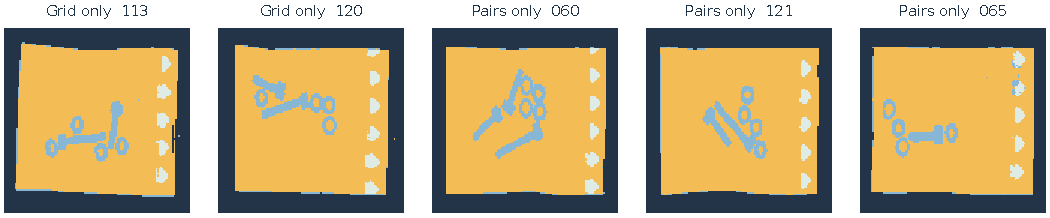
\includegraphics[width=.88\textwidth]{screw_discordant.pdf}
\caption{\textbf{Screw-bag logical cases with discordant grid and centroid-pair alarms.} At the pre-specified thresholds, two of 79 supported faults alarm under the grid alone and three under the pair summary alone. The colorized maps show the five cases. Thin fragments around the bag and merged foreground illustrate the difference between predicted counts and physical screw inventory.}
\label{fig:screw}
\end{figure*}

The matched screw-bag cohort has 79 faults and 95 good maps. Pairs trail the grid by 17.1 points [$-24.9$, $-9.0$] from unrounded scores (17.2 from rounded table entries). The other three categories average about $-0.3$ points. Adding placement and extent gives 56.6\% versus 58.3\% for the original pair block and 75.5\% for the grid. The paired difference relative to the original pair block is $-1.7$ points [$-9.9$, $+6.3$]. In \cref{fig:screw}, the predicted metal role includes narrow boundary fragments and can merge physical parts. For example, the largest projected long-axis extent in case 121 belongs to a 143-pixel fragment along the image-side edge. Per-role pooled extent therefore cannot identify the actual length of each screw. This probe supports a limit of the tested summaries on the supplied maps. In the native full comparison the grid's logical recall is 51.5\% macro with 11.1\% good alarms, versus 53.3\% and 10.3\% for the bag. Matched SALAD minus grid is $+3.0$ points [$-2.1$, $+8.2$] across the four supported categories and $+15.1$ [5.9, 24.5] in screw bag.

\section{Exploratory SVC--PA query}
The code comparison keeps five negative fit patients, 20 negative calibration patients, and test patients with 24 Glenn codes and ten without. Mask face contact has 100\% test AUROC, detects 24/24 positives [85.8, 100], and alarms on 1/10 code-negative scans [0.25, 44.5]. The $31.47\,\mathrm{mm}^2$ calibration threshold is below the largest negative ($48.45$) and smallest positive ($58.17$). Axial-mask profiles detect 21/24 with zero negative alarms. Full contextual loss has 19.6\% AUROC and detects 0/24 at its cutoff. Its masked link probability is higher on the Glenn-coded test scans (median 0.712 versus 0.441). Refitting without the degree terms raises AUROC to 44.2\%. Removing the shared-neighbor terms gives 18.3\%. Distance alone gives 75.4\%. Removing one incident link at a time while holding the SVC--PA bit fixed yields mean absolute within-patient probability shifts of 0.093 on the 21 Glenn-coded patients with at least one such link and 0.144 on ten code-negative patients. These are exploratory sensitivity checks on five fit patients and a single query. They do not resolve the causal effects of surgery. Five target-negative SVC variants occur in the release, with two in fit and three in calibration. The test has zero. Independent adjudication of native relations and benign variants is needed to extend the scope beyond this code.

\section{Data use}
The medical experiments use existing de-identified research releases and their original labels, and constitute a secondary analysis without new ethics review, participant recruitment, intervention or consent collection. The HVSMR authors report approval by the Boston Children's Hospital IRB with a waiver of written consent~\cite{pace2024}. The photographs derive from the public MVTec LOCO AD dataset, distributed under CC BY-NC-SA 4.0, and derived image panels retain this attribution and license. Selected pairs, data splits, scores, calibration sets, checkpoint hashes and figure inputs are released with the code.

\section*{LLM Usage Statement}
OpenAI Codex was used to develop and implement the revision experiments, run and check the code, inspect public sources and data provenance, produce figures and tables from recorded outputs, and draft and edit the main text and supplementary material. Anthropic Claude was used to restructure and edit the text and to redraw the figures from the recorded outputs. Photograph edits are deterministic composites of the stated dataset assets.

{\small
\bibliographystyle{ieeenat_fullname}
\bibliography{references}
}
\end{document}
